\section{System Overview}
\label{sec:system}

\begin{figure}
\centering
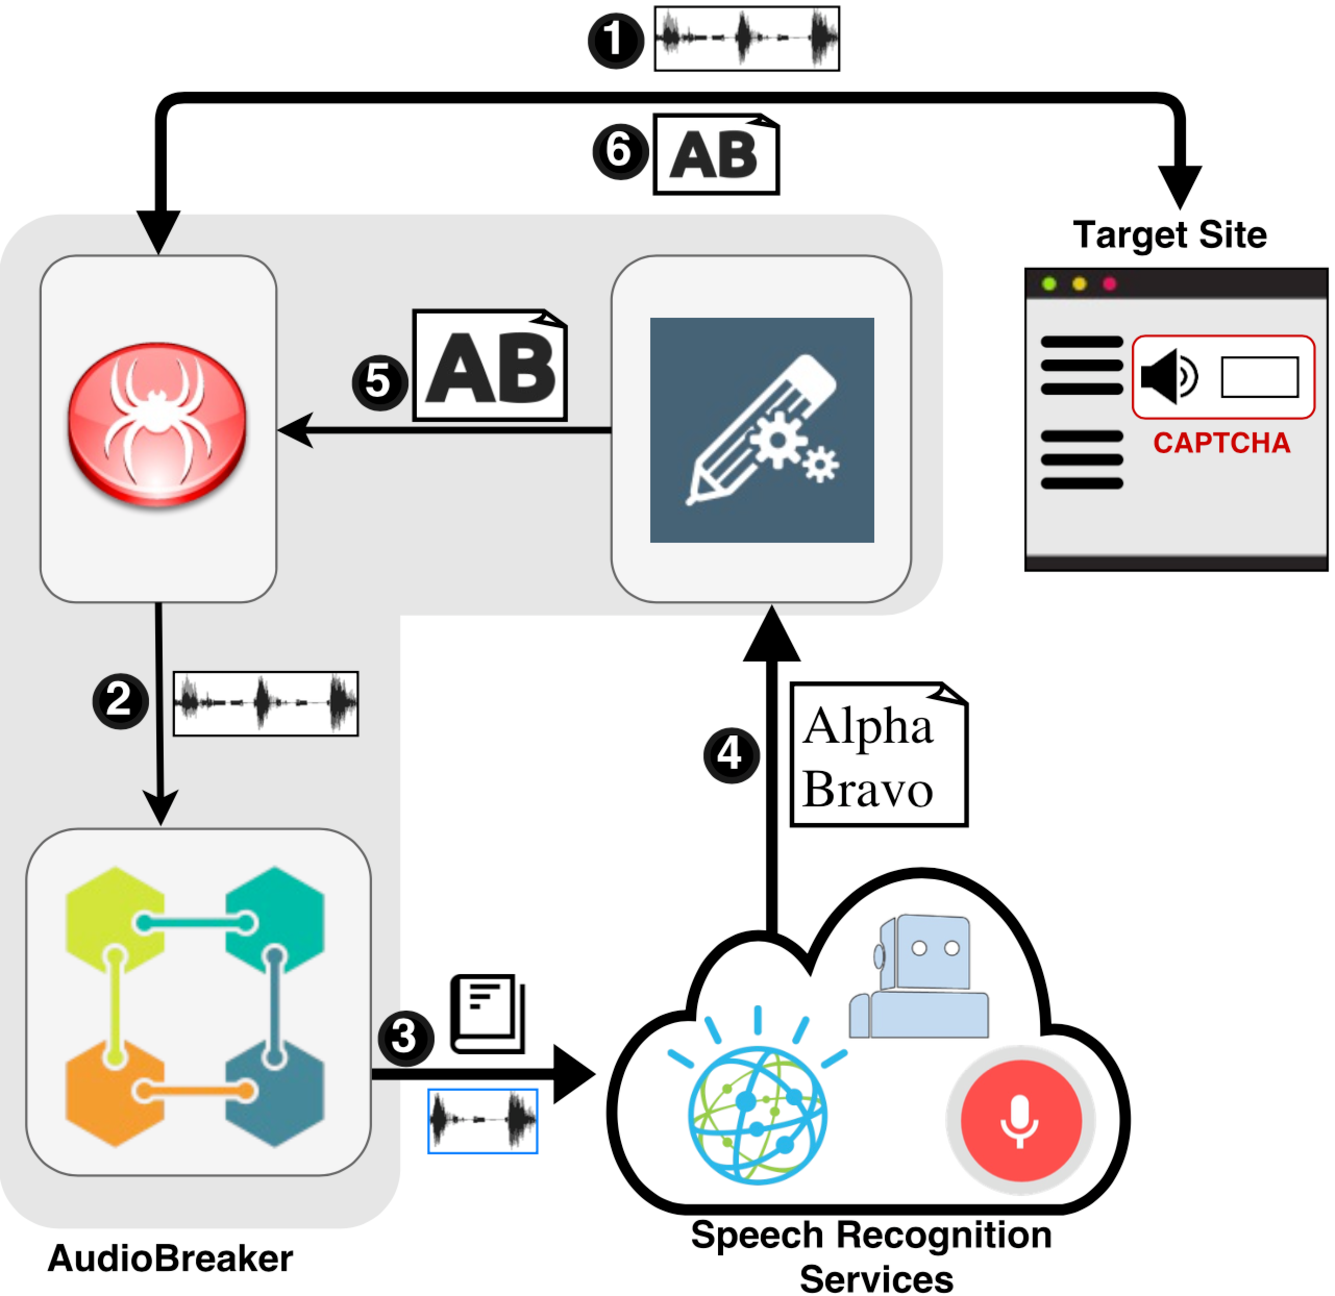
\includegraphics[width=\columnwidth]{figures/breaker_arch.pdf}
\caption{Overview of the \system system and the captcha-solving workflow..}
\label{fig:breaker}
\end{figure}

In this section we first present an overview of \system's design and describe the automated 
captcha-solving process. We then offer more details on our system's implementation.

\subsection{\system Design}

One of the main goals of our work is to explore the effectiveness of different speech recognition
services against a large number of different audio captcha services. To that end, we opted for 
a modular design for \system, as that provides flexibility in adding support for new captcha 
systems and speech recognition APIs. Our system is comprised of 3 basic components. The main 
component is responsible for the browser automation and handles all browser-related actions,
including crawling and rendering webpages, extracting the audio captchas, and providing the solutions
to the challenges. It also performs specific actions to mimic a user's steps and avoid triggering  
checks implemented by the captcha services for detecting bots (e.g., mouse over actions, or text 
box highlighting before solutions are input).
The second component completes some pre-processing and configuration steps 
necessary before the audio recordings are passed to the speech recognition services. The final 
component handles the post-processing of the transcribed text for preparing the solution that will
be submitted to the captcha service.

Figure~\ref{fig:breaker} presents the main components of \system and outlines the workflow of
an automated attack against a target website that protects a specific action with a captcha 
service that also supports audio challenges.

\protect\circlea{\small 1} Our system visits a webpage that offers the desired functionality 
(e.g., account creation, message posting, etc.). After identifying the captcha element within 
the page, the audio challenge is extracted.

\protect\circlea{\small 2} The audio file is passed to the pre-processing component, which is responsible 
for preparing the audio file that will be passed to the speech recognition service. If there are audio 
instructions at the beginning of the audio challenge they are removed, and the final audio
recording is then converted to a supported format. Then, based on the captcha service, our system
selects the speech recognition service with the best results for the specific challenge.

\protect\circlea{\small 3} The audio file is uploaded for transcription by the module that handles that solver, 
together with a predetermined configuration. The configuration allows us to fine-tune the "transcript"ion process
for better results; specifically we restrict the dictionary used by the solver (e.g., to only expect  
numbers) as well as the accent classifier to use (services may support multiple English accents 
-- British, American etc.).

\protect\circlea{\small 4} The transcription of the audio challenge is obtained from the solver 
and passed to the post-processing component. The corresponding module will process the transcription 
based on a set of rules %(e.g., based on the captcha's dictionary and common homophones) 
and prepare the solution to the challenge. If a service employs the 
NATO phonetic alphabet, the transcribed words will be mapped to the letters they represent. For instance, 
``Alpha Bravo'' will be substituted with ``AB''. Furthermore, we have manually prepared rulesets
per captcha service and speech recognition engine %for further processing the transcriptions. This processing
that handle cases of homophones or recurring mis-identifications; for instance, $\{two,too,to\}$ are all
mapped to $\{2\}$ for captcha services that only contain digits in the audio challenges.

\protect\circlea{\small 5} The final solution is forwarded to the browser automation module,
which is responsible for passing the captcha challenge.

\protect\circlea{\small 6} The browser automation module inputs the solution while mimicking 
user behavior, as certain captcha services have deployed extra checks for identifying bots.
It also verifies that the solution was accepted by the captcha service.

\subsection{Implementation Details}

\textbf{Browser automation.}
Our browser automation component is built upon the Selenium framework~\cite{selenium}. This offers
flexibility in setting up our environment (e.g., browser), as well as advanced functionality
and configurability that allow us to implement scraping behavior that does not trigger bot detection
mechanisms currently deployed by certain services.\footnote{There is no straightforward way to detect 
automation apart for checking some predefined variables (which can be easily modified).}
%Most websites do not check these in practice.}.
Selenium communicates with the browser via a special protocol 
native to each browser, and has access to everything loaded for the visited web site, including all Javascript, DOM 
elements and even ``Secure'' HTTP cookies. The special protocol is required for communication with the browser,
and enables execution of the automation scripts without violating the same origin policy.
%In more detail, a sandbox is created for
%every website the browser creates a sandbox for the website's javascript, this way the javascript that 
%belongs to one website does not execute on another website that is currently loaded on the browser. 
%(more detail on cross site scripting). To overcome this 
Specifically, Selenium acts as an HTTP Proxy server when
the browser is launched through Selenium scripts, and Javascript (Selenium Core) is injected into the browser;
all subsequents requests are then handled through Selenium. In essence, the browser perceives the
web page as being served from Selenium's domain rather than the actual web server hosting the website.
As such, the automation scripts appear to belong to the same origin with the web page. This approach, 
however, faces certain limitations, which are handled by ``WebDriver'' an object oriented API
%as the Core is limited by the JavaScript sandbox of 
%the browser (Due to same origin policy). The Webdriver, 
which handles the browser from outside. 
%This was 
%the marked difference between Selenium 1.0 and Selenium 2.0 as by being limited by the sandbox and therefore 
%has reduced functional test coverage. 


\note{how do you automatically identify the captcha service being used on a random page?}

\textbf{Speech recognition APIs.}
We have incorporated support for three widely-available voice recognition services: Google's Cloud Speech API,
IBM Watson's Text-to-Speech API, and Facebook's Wit.ai service. Below we 
provide some details regarding these services.

\begin{lstlisting}[language=json,firstnumber=1,caption={Example response from IBM Watson's API for an audio challenge from Google \re v2.a.},label={lst:IBM}]
{
results: [
{alternatives: [{transcript:"eight", confidence:0.982679}]},
{alternatives: [{transcript:"three", confidence:0.742102}]},
{alternatives: [{transcript:"eight", confidence:0.593190}]},
{alternatives: [{transcript:"nine", confidence:0.6004673}]},
{alternatives: [{transcript:"five", confidence:0.982679}]}
]
}

\end{lstlisting}

\emph{IBM Bluemix (Watson).} IBM Watson's Speech To Text service provides a public REST API, and the website provides 
sample code in multiple programming languages to facilitate integration.
%in Curl, Ruby and Node.JS with best practices for using their REST API. The API is also very well documented.
The service accepts various audio file formats as input, and returns a JSON object
with the timestamps of each recognized word, a confidence score, and alternative hypothesis (if there is 
another interpretation for the word). It provides support for various languages 
like Spanish, Brazilian, Mandarin, Arabic, and two different accents in English - British and American.
%is available for free for the first 1000 min/per month for each 
%account, after which each additional minute is charged \$0.02. We used multiple accounts each to access the free 
%version of the software for the term of our project.

\emph{Wit.} Wit, which was acquired by Facebook in 2015, offers an API that leverages their natural language processing
capabilities and is geared towards developers building voice-activated interfaces (e.g., for home automation). We transform 
audio files to a WAV format (if required) in a monophonic (\emph{mono}) form as Wit does not currently support stereo format.
We use the ``free-text'' and ``keywords'' search strategies, that allow us \note{to identify values belonging to a predefined 
list of keywords}.

\emph{Google Cloud Speech.}  Google has released a RESTful API that offers access to a speech recognition system built on 
a deep learning neural network that can identify speech in over 80 languages. The API endpoint for recognizing speech supports
the ``phrases'' optional argument that allows us to narrow down the keywords their classifier model tries to identify, which 
results in higher accuracy against captcha schemes that use limited/restricted vocabularies (e.g., only digits). The Google
speech API also requires a mono form, and supports both WAV and FLAC file formats.

%// Multiple entities allowed per field -- separated with ";"
\begin{lstlisting}[language=json,firstnumber=1,mathescape=true,caption={Subset of rules used by our post-processing component for
converting keywords in the transcription to the required transformation for the captcha's solution.},label={lst:rules}]
// "*" works as a wildcard. 
// [Captcha, Speech API]: {keywords} $\longmapsto$ "transformation"

// Phase 1
[BotDetect, *]: {hey,hay} $\longmapsto$ "a"
[BotDetect, IBM]: {three,through,tree,free,he,green} $\longmapsto$ "3"
[BotDetect, Wit]: {bee,be} $\longmapsto$ "b"
[CaptchasNet, Wit]: {gulf} $\longmapsto$ "golf"
[CaptchasNet, Wit]: {elsa} $\longmapsto$ "alpha"

// Phase 2
[*, *]: {alpha} $\longmapsto$ "a"
[*, *]: {bravo} $\longmapsto$ "b"
\end{lstlisting}

\textbf{Post-processing.} Our post-processing component relies on a set of manually created rules that define transformations
of the transcribed audio to the string that will eventually be provided by our main component as the answer to the audio challenge.
These rules were created after extensive manual experimentation with each speech recognition service for each captcha scheme,
by determining mis-identified words that are homophones or sound somewhat similar to keywords that belong to the 
restricted dictionary of each captcha scheme (apart from Microsoft Live that uses common English words). This was motivated
by our observation of recurring mistakes that were made by each speech recognition service (some of which were common across
all three engines), which can be attributed to the ``consistent'' type of distortion and noise in each captcha system.

In Listing~\ref{lst:rules} we provide a few examples of our transformation rules. In the first phase, the rules process the 
transcription and apply transformations based on homophones or recurring mistakes that we have identified. For instance, 
the number ``3'' can me mis-labelled by the speech recognition service as ``tree'' that sounds similar.
Any keywords that have not been transformed are handled by the more generic rules of phase 2, e.g., mapping 
words form the NATO phonetic alphabet to their corresponding letter.

